\subsection{Event identification of $d(K^-, p)$ events}
\begin{figure}[htbp]
  \centering
  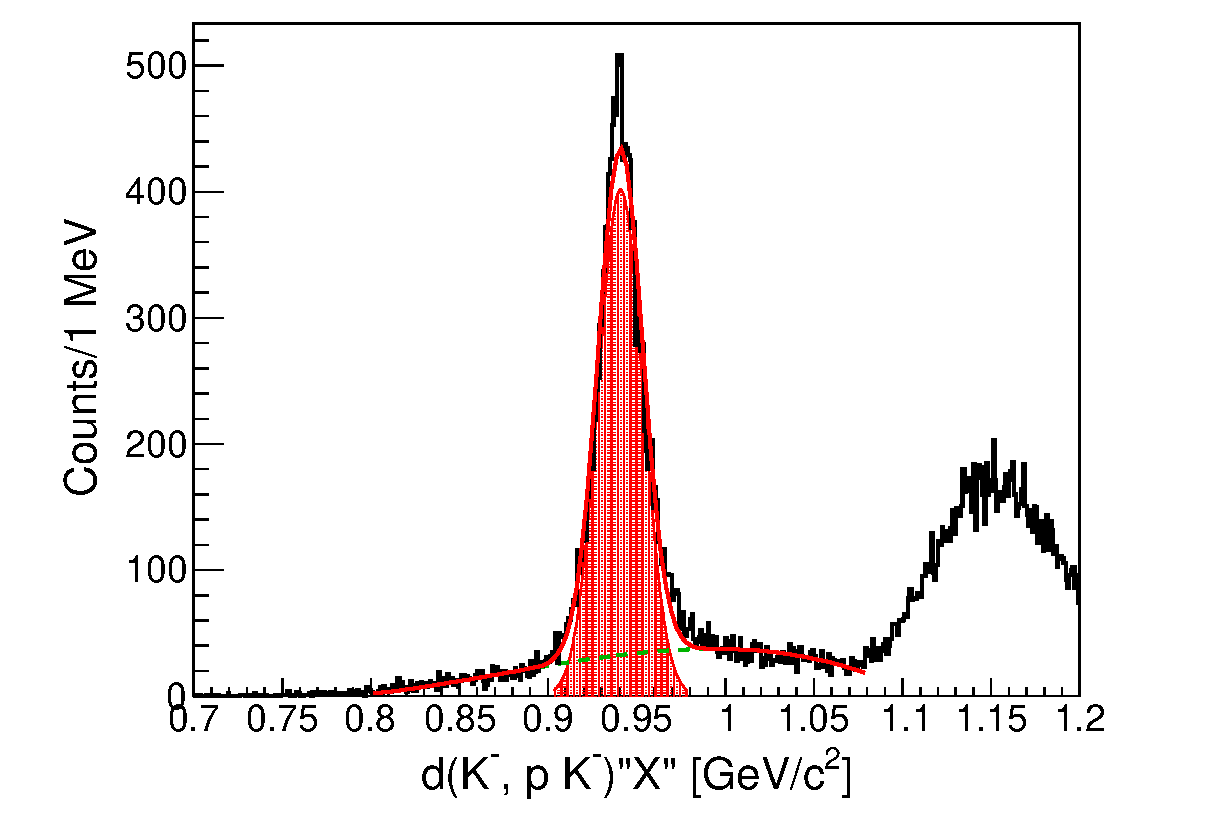
\includegraphics[width=8cm]{../pic/Run68/KP_ana/KPkm_MM.eps}
  \caption{
    This figure shows $d(K^-, p K^-)$ missing mass spectrum in forward proton and $K^-$ tagged events.
    Red line is whole fitting result and red hatch indicates fitting gaussian.
    Background was estimated 3rd order polynomial function which indicates green dotted line.
  }
  \label{fig:KPkm_MM}
\end{figure}

We use the $d(K^-, p K^-)"n"$ for the time offset calibration.
The missing $n$ peak was clearly seen in Fig\ref{fig:KNkm_MM}
